\documentclass[11pt,a4paper]{report}
\usepackage{marvosym}

\assignment{3}
\group{...}
\students{..........}{..........}

\begin{document}

\maketitle

\section{Search Algorithms and their relations (3 pts)}
Consider the maze problems given on Figure 1. The goal is to find a path from \Gentsroom ~ to \EURhv ~ moving up, down, left or right. The black cells represent walls. This question must be answered by hand and doesn't require any programming.

\begin{enumerate}
\item Give a consistent heuristic for this problem. Prove that it is consistent. Also prove that it is admissible. \textbf{(1 pt)}
\end{enumerate}

\begin{answers}[4cm]
% Your answer here
\end{answers}



\begin{enumerate}
\setcounter{enumi}{1}
\item Show on the left maze the states (board positions) that
are visited when performing a uniform-cost graph search, by writing the order numbers in the relevant cells. We assume that when different states in the fringe have the smallest value, the algorithm chooses the state with the smallest coordinate $(i,j)$ ($(0,0)$ being the bottom left position, $i$ being the horizontal index and $j$ the vertical one) using a lexicographical order. \textbf{(1 pt)}
\end{enumerate}

\begin{answers}[5.2cm]
% Your answer here
\begin{center}
\resizebox{5cm}{!}{
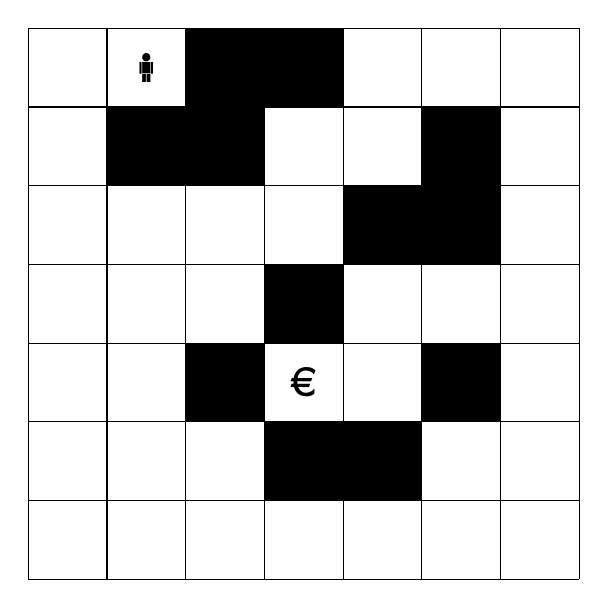
\begin{tikzpicture}
         \draw (0,0) grid (7, 7);
	   
	   \fill (2, 7) rectangle (4, 6);
	   \fill (1, 6) rectangle (2, 5);
	   \fill (2, 7) rectangle (3, 5);
          \fill (4, 5) rectangle (6, 4);
          \fill (5, 6) rectangle (6, 4);
   	 \fill (3, 4) rectangle (4, 3);
	   \fill (2, 3) rectangle (3, 2);
	   \fill (3, 2) rectangle (5, 1);
	   \fill (5, 2) rectangle (6, 3);
          
          \node at (1.5, 6.5) {\Large \Gentsroom};
          \node at (3.5, 2.5) {\Large \EURhv};
        \end{tikzpicture}
}
\end{center}
\end{answers}



\begin{enumerate}
\setcounter{enumi}{2}
\item Show on the right maze the board positions visited by $A^{\star}$ graph search with a manhattan distance heuristic (ignoring walls), by writing the order numbers in the relevant cells. A state is visited when it is selected in the fringe and expanded. When several states have the smallest path cost, they are visited in the same lexicographical order as the one used for uniform-cost graph search. \textbf{(1 pt)}
\end{enumerate}

\begin{answers}[5.2cm]
% Your answer here
\begin{center}
\resizebox{5cm}{!}{
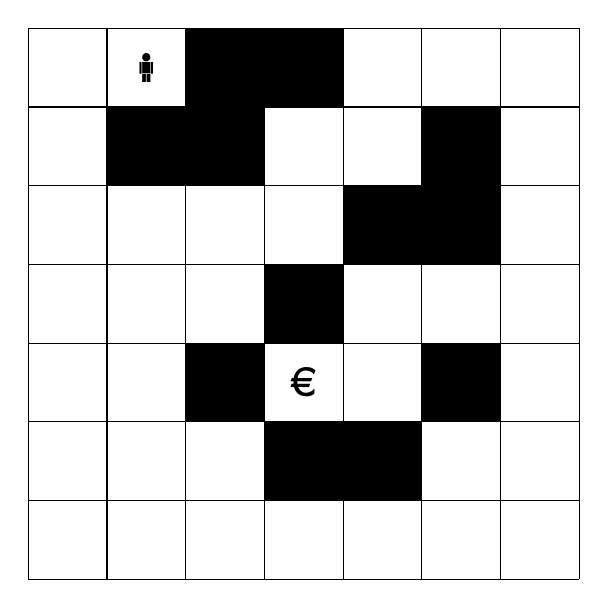
\begin{tikzpicture}
         \draw (0,0) grid (7, 7);
	   
	   \fill (2, 7) rectangle (4, 6);
	   \fill (1, 6) rectangle (2, 5);
	   \fill (2, 7) rectangle (3, 5);
          \fill (4, 5) rectangle (6, 4);
          \fill (5, 6) rectangle (6, 4);
   	 \fill (3, 4) rectangle (4, 3);
	   \fill (2, 3) rectangle (3, 2);
	   \fill (3, 2) rectangle (5, 1);
	   \fill (5, 2) rectangle (6, 3);
          
          \node at (1.5, 6.5) {\Large \Gentsroom};
          \node at (3.5, 2.5) {\Large \EURhv};
        \end{tikzpicture}
}
\end{center}
\end{answers}




\section{N-Amazons problem (8 pts)}

\begin{enumerate}
  \item Model the N problem as a search problem; describe: \textbf{(2 pts)}
		\begin{itemize}
			\item States
			\item Initial state
			\item Actions / Transition model
			\item Goal test
			\item Path cost function
		\end{itemize}
\end{enumerate}

\begin{answers}[8cm]
% Your answer here
\end{answers}


\newpage
\begin{enumerate}
\setcounter{enumi}{1}
\item Give an upper bound on the number of different states for an N-Amazons problem with N=n. Justify your answer precisely. \textbf{(0.5 pt)}
\end{enumerate}

\begin{answers}[5cm]
% Your answer here
\end{answers}



\begin{enumerate}
\setcounter{enumi}{2}
\item Give an admissible heuristic for a N=n. Prove that it is admissible. What is its complexity ? \textbf{(1 pts)}
\end{enumerate}

\begin{answers}[5cm]
% Your answer here
\end{answers}



\begin{enumerate}
\setcounter{enumi}{4}
\item \textbf{Implement} your solver. Extend the \emph{Problem} class and implement 
		the necessary methods and other class(es) if necessary.  \textbf{(0.5 pt)}
\item \textbf{Experiment}, compare and analyze informed (\emph{astar\_graph\_search}), uninformed \\
    (\emph{breadth\_first\_graph\_search} and \emph{depth\_first\_graph\_search}) graph search of aima-python3 on N = [10, 11, 12, 13, 20, 25, 30]. \textbf{(3 pts for the whole question)}
		
		Report in a table the time and the number of explored nodes and the number of 
		steps to reach the solution.
		
		Are the number of explored nodes always smaller with 
		\emph{astar\_graph\_search}? 
		What about the computation time? 
		Why? 
		 
		 When no solution can be found by a strategy in a reasonable time (say \textbf{3 
		 min}), indicate the reason (time-out and/or exceeded the memory).
\end{enumerate}

\begin{answers}[8cm]
% Your answer here

\end{answers}

~ 

\begin{answers}[6.5cm]
\begin{center}
\begin{tabular}{||l||l|l|l||l|l|l||l|l|l||l|l|l||}
\hline
\multirow{3}{*}{Inst.} & \multicolumn{3}{c||}{$A^{\star}$ Graph}& \multicolumn{3}{c||}{BFS Graph} & \multicolumn{3}{c||}{DFS Graph}\\
 & NS & T(s) & EN & NS & T(s) & EN & NS & T(s) & EN\\
\hline
i01 & & & & & & & & & \\
\hline
i02 & & & & & & & & & \\
\hline
i03 & & & & & & & & & \\
\hline
i04 & & & & & & & & & \\
\hline
i05 & & & & & & & & & \\
\hline
i06 & & & & & & & & & \\
\hline
i07 & & & & & & & & & \\
\hline
i08 & & & & & & & & & \\
\hline
i09 & & & & & & & & & \\
\hline
i10 & & & & & & & & & \\
\hline
\end{tabular}\\

~\\
\textbf{NS}: Number of steps — \textbf{T}: Time — \textbf{EN}: Explored nodes
\end{center}
\end{answers}



\begin{enumerate}
\setcounter{enumi}{5}
\item \textbf{Submit} your program on INGInious, using the \textit{A*} algorithm with your best heuristic(s).
		 Your file must be named \emph{namazon.py}. 
      Your program should be able to, given an integer as argument, return the correct output.
		 Your program must print to the standard output a solution to the N's given in argument for the N-Amazons problem, satisfying the described output format. \textbf{(2 pts)}
\end{enumerate}

\begin{answer}
% ANY COMMENTS ABOUT YOUR CODE
\end{answer}

\section{Local Search: Sudoku Problem (8 pts)}

\begin{enumerate}
    \item Formulate the Sudoku problem as a Local Search problem (problem, cost function, feasible solutions, optimal solutions). \textbf{(2 pts)}
\end{enumerate}

\begin{answer}

\end{answer}

\begin{enumerate}
    \item You are given a template on Moodle: \url{sudoku.py}. Implement your own simulated annealing algorithm and your own \url{objective\_score} function. Your program will be evaluated in on 15 instances (during 3 minutes each) of which 5 are hidden. We expect you to solve (get the optimal solution) at least 12 out of the 15. \textbf{(6 pt)}
\end{enumerate}

\begin{answer}
 % ANY COMMENTS ABOUT YOUR CODE   
\end{answer}
\end{document}